\subsection{Image Meter - Messen im Foto}

\subsubsection{Vorstellung}
Die App \im{} von \emph{Dirk Farin} hat zur Zeit des Downloads (20. Januar 2018) bei insgesamt 2.764 abgegeben Bewertungen eine durchschnittliche Bewertung von 3,9 von 5 Sternen im Google Play-Store \citep{FarinIM}.
Hierbei haben 72\% (1324 + 654) der Bewertungen vier oder fünf, und nur 28\% (289 + 154 + 343) 3 oder weniger Sterne. \\
Dies ist im Vergleich zu den aderen Apps, die im Play-Store unter dem Suchbegriff ``Aufmaße'' frei erhältlich sind, eine vergleichweise hohe Bewertung, und macht diese App zu einer der beliebtesten in der Kategorie \emph{Aufmaße}.
Selbst beschreibt der Entwickler die App im Play-Store wie folgt \citep{FarinIM}:

\begin{quote}
  ``ImageMeter erlaubt das Beschriften Ihrer Fotos mit Längen-, Winkel- und Flächenmaßen sowie Text.
  Das ist viel einfacher und anschaulicher als aufwändig eine Skizze zu zeichnen.''
\end{quote}

\noindent
Beim Start der App wird dem Benutzer der sogenannte ``Tipp des Tages'' angezeigt. \\

\begin{wrapfigure}{R}{0.5\textwidth}
  \centering
  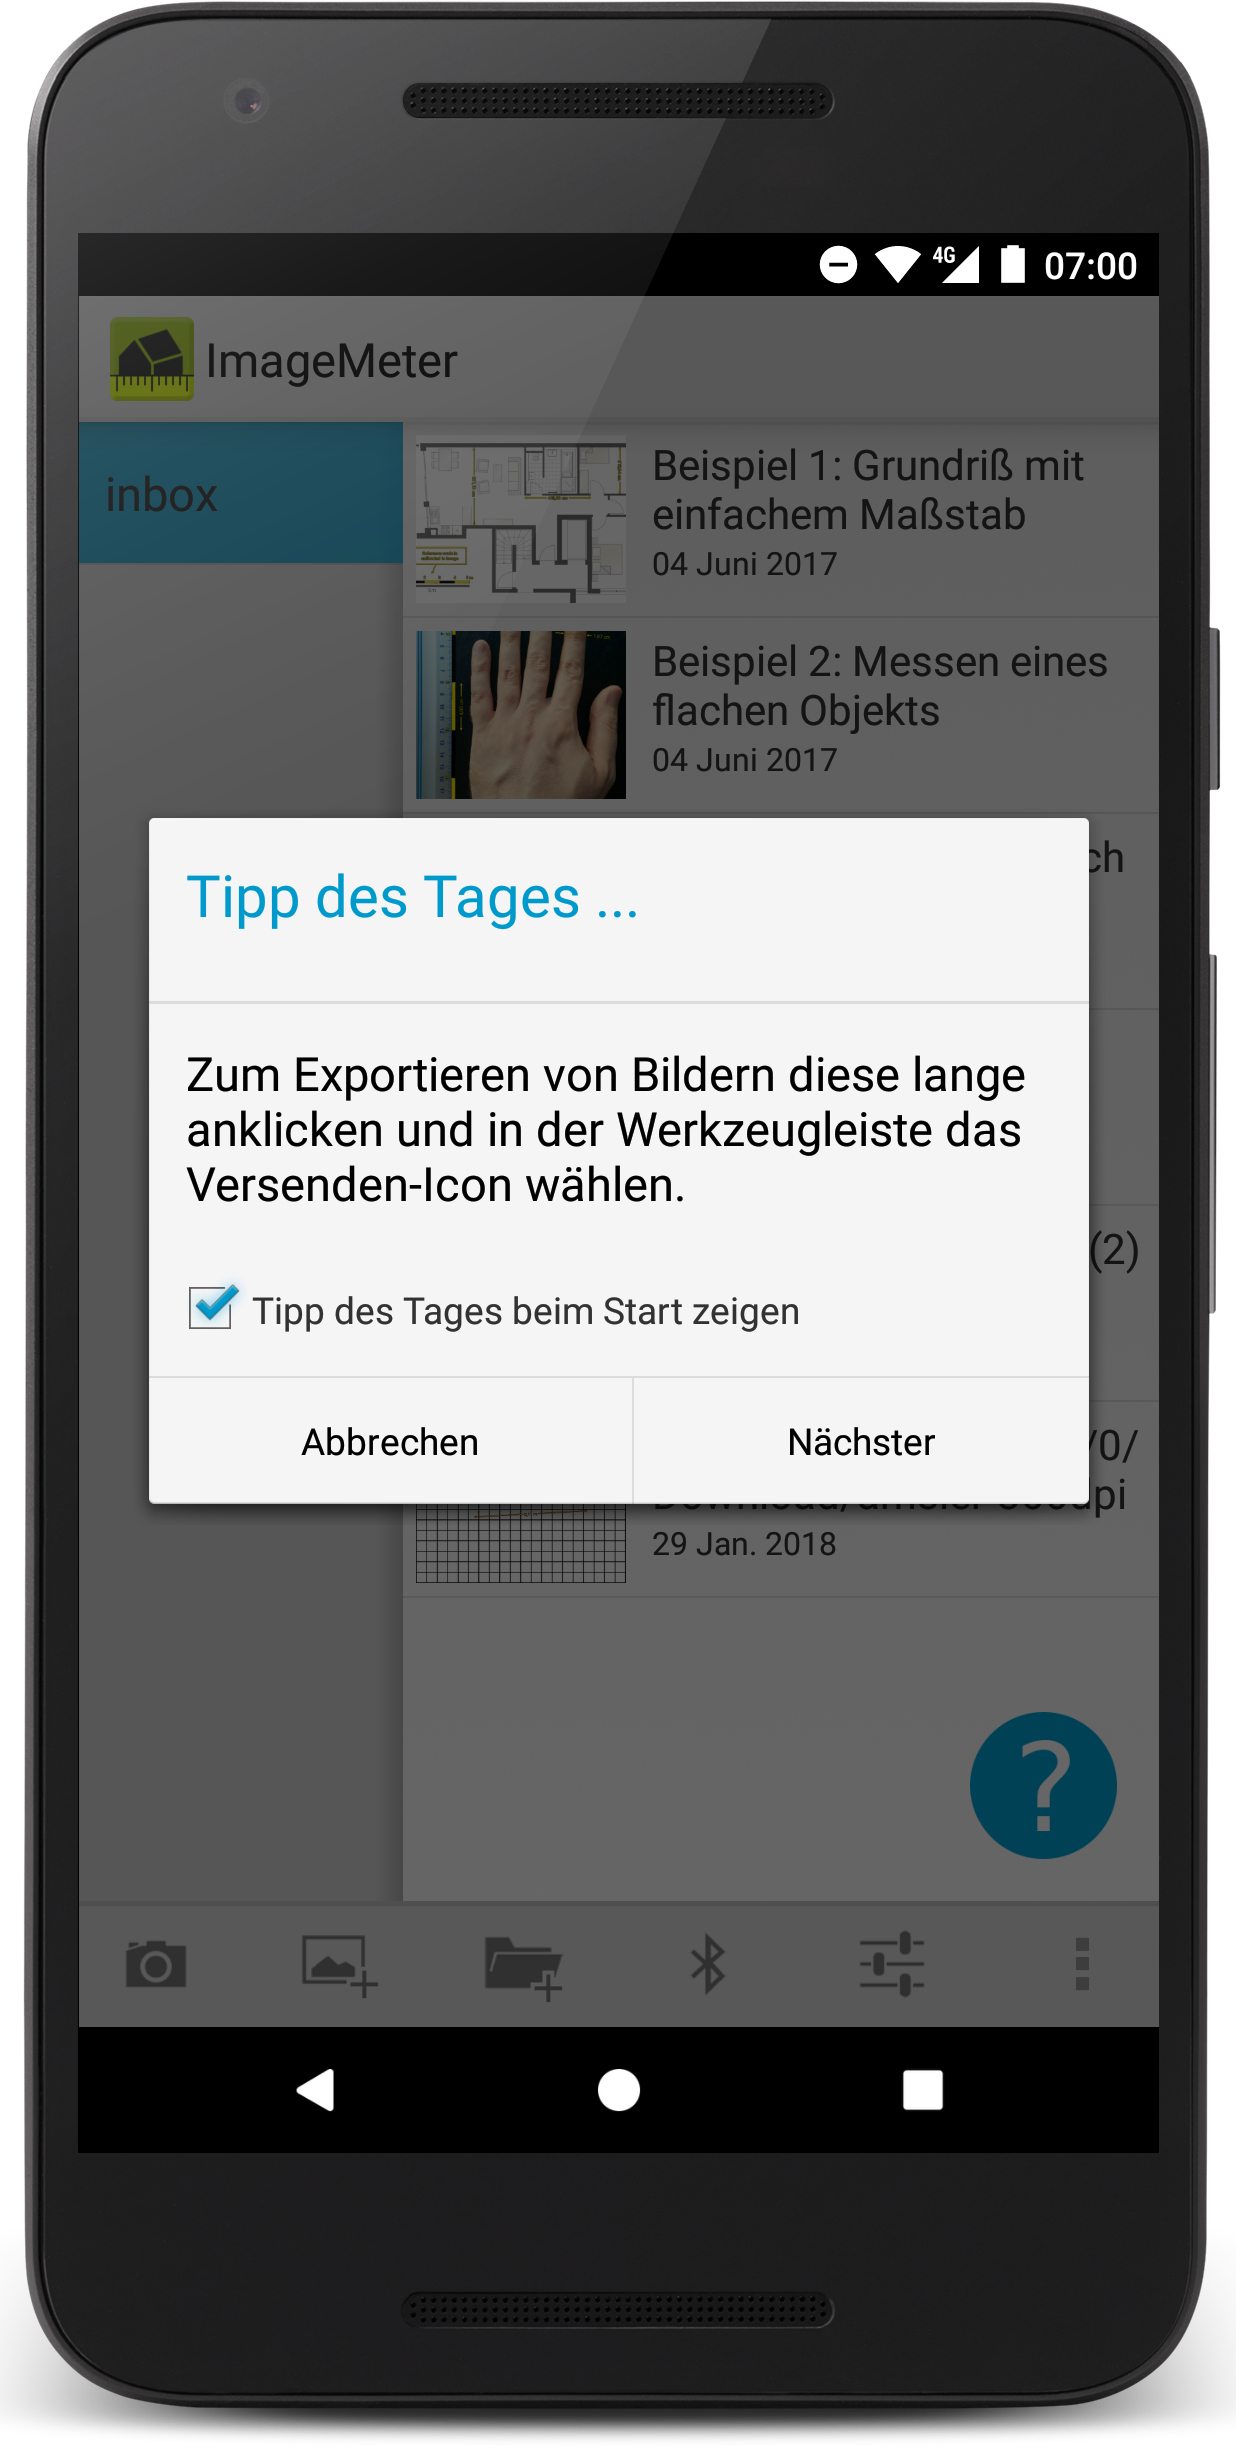
\includegraphics[keepaspectratio, width=0.5\textwidth]{image_meter/tip}
  \caption{``Tipp des Tages'' beim Start der App}
  \label{fig:imtip}
\end{wrapfigure}

Dieser enthält Informationen zu bestimmten Funktionen der App, wie zum Beispiel dem Exportieren von Bildern (siehe \autoref{fig:imtip}).
Hier hat der Nutzer die Möglichkeit sich weitere Tipps anzusehen, oder diese durch das Entfernen des Hakens in der Checkbox ``Tipp des Tages beim Start zeigen'' dauerhaft zu deaktivieren. \\

Sobald der Dialog zum ``Tipp des Tages'' geschlossen wurde, bietet sich über die Aktionsleiste am unteren Bildschirmrand die Möglichkeit, ein neues Bild aufzunehmen, oder direkt eines aus der Galerie zu importieren (siehe \autoref{fig:immenu}).
Das ausgewählte Bild wird nach erfolgreichem Import in die App im Hauptmenü an die Bilderliste angehangen. \\

Hier gelangt der Benutzer durch einen Klick auf das gewünschte Bild in eine neue Bildschirmöberfläche, in der Aufmaße eingezeichnet werden können (siehe \autoref{fig:imdraw})
In dieser Umgebung wird zusätzlich zum Bild noch eine Statusleiste am unteren Bildschirmrand und ein darüber befindlicher ``Floating Action Button'' \todo{ref} mit einem Fragezeichen-Symbol angezeigt.
Beim Klick auf diesen schwebenden Button öffnet sich eine Hilfe-Seite, in der zu den verschiedenen Funktionalitäten der App häufig gestellte Fragen, und deren Antworten zu lesen sind. \\

Zusätzlich zu dieser Hilfestellung, wird dem Benutzer beim Auswählen des ``Zeichen-Modus'' ein erklärender Text über der Statusleiste angezeigt (siehe \autoref{fig:imdraw}), der genau beschreibt, welche Aktion der Nutzer in diesem Systemzustand durchführen kann bzw. soll. \\

\begin{figure}[h]
  \centering
  \begin{subfigure}[t]{0.4\textwidth}
    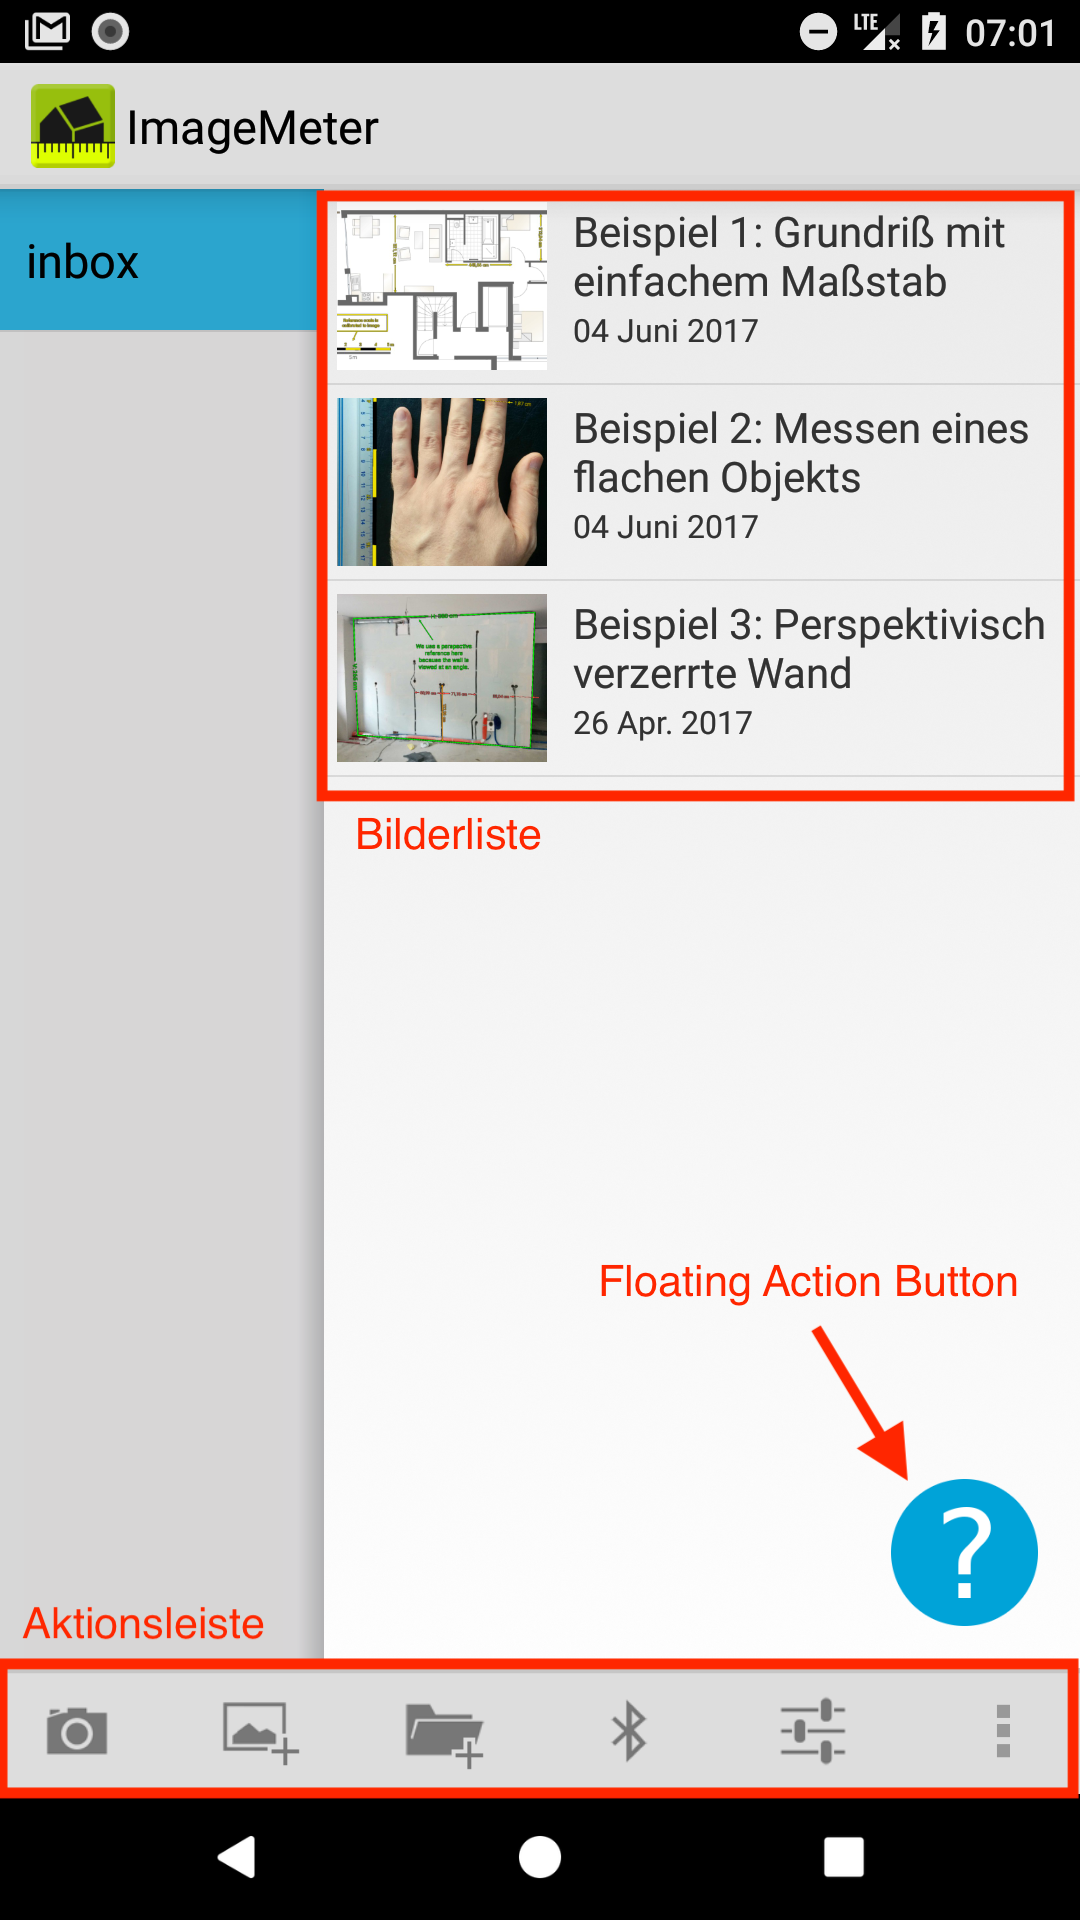
\includegraphics[keepaspectratio, width=\textwidth]{image_meter/menu}
    \caption{Hauptansicht der App}
    \label{fig:immenu}	
  \end{subfigure}
  \begin{subfigure}[t]{0.4\textwidth}
    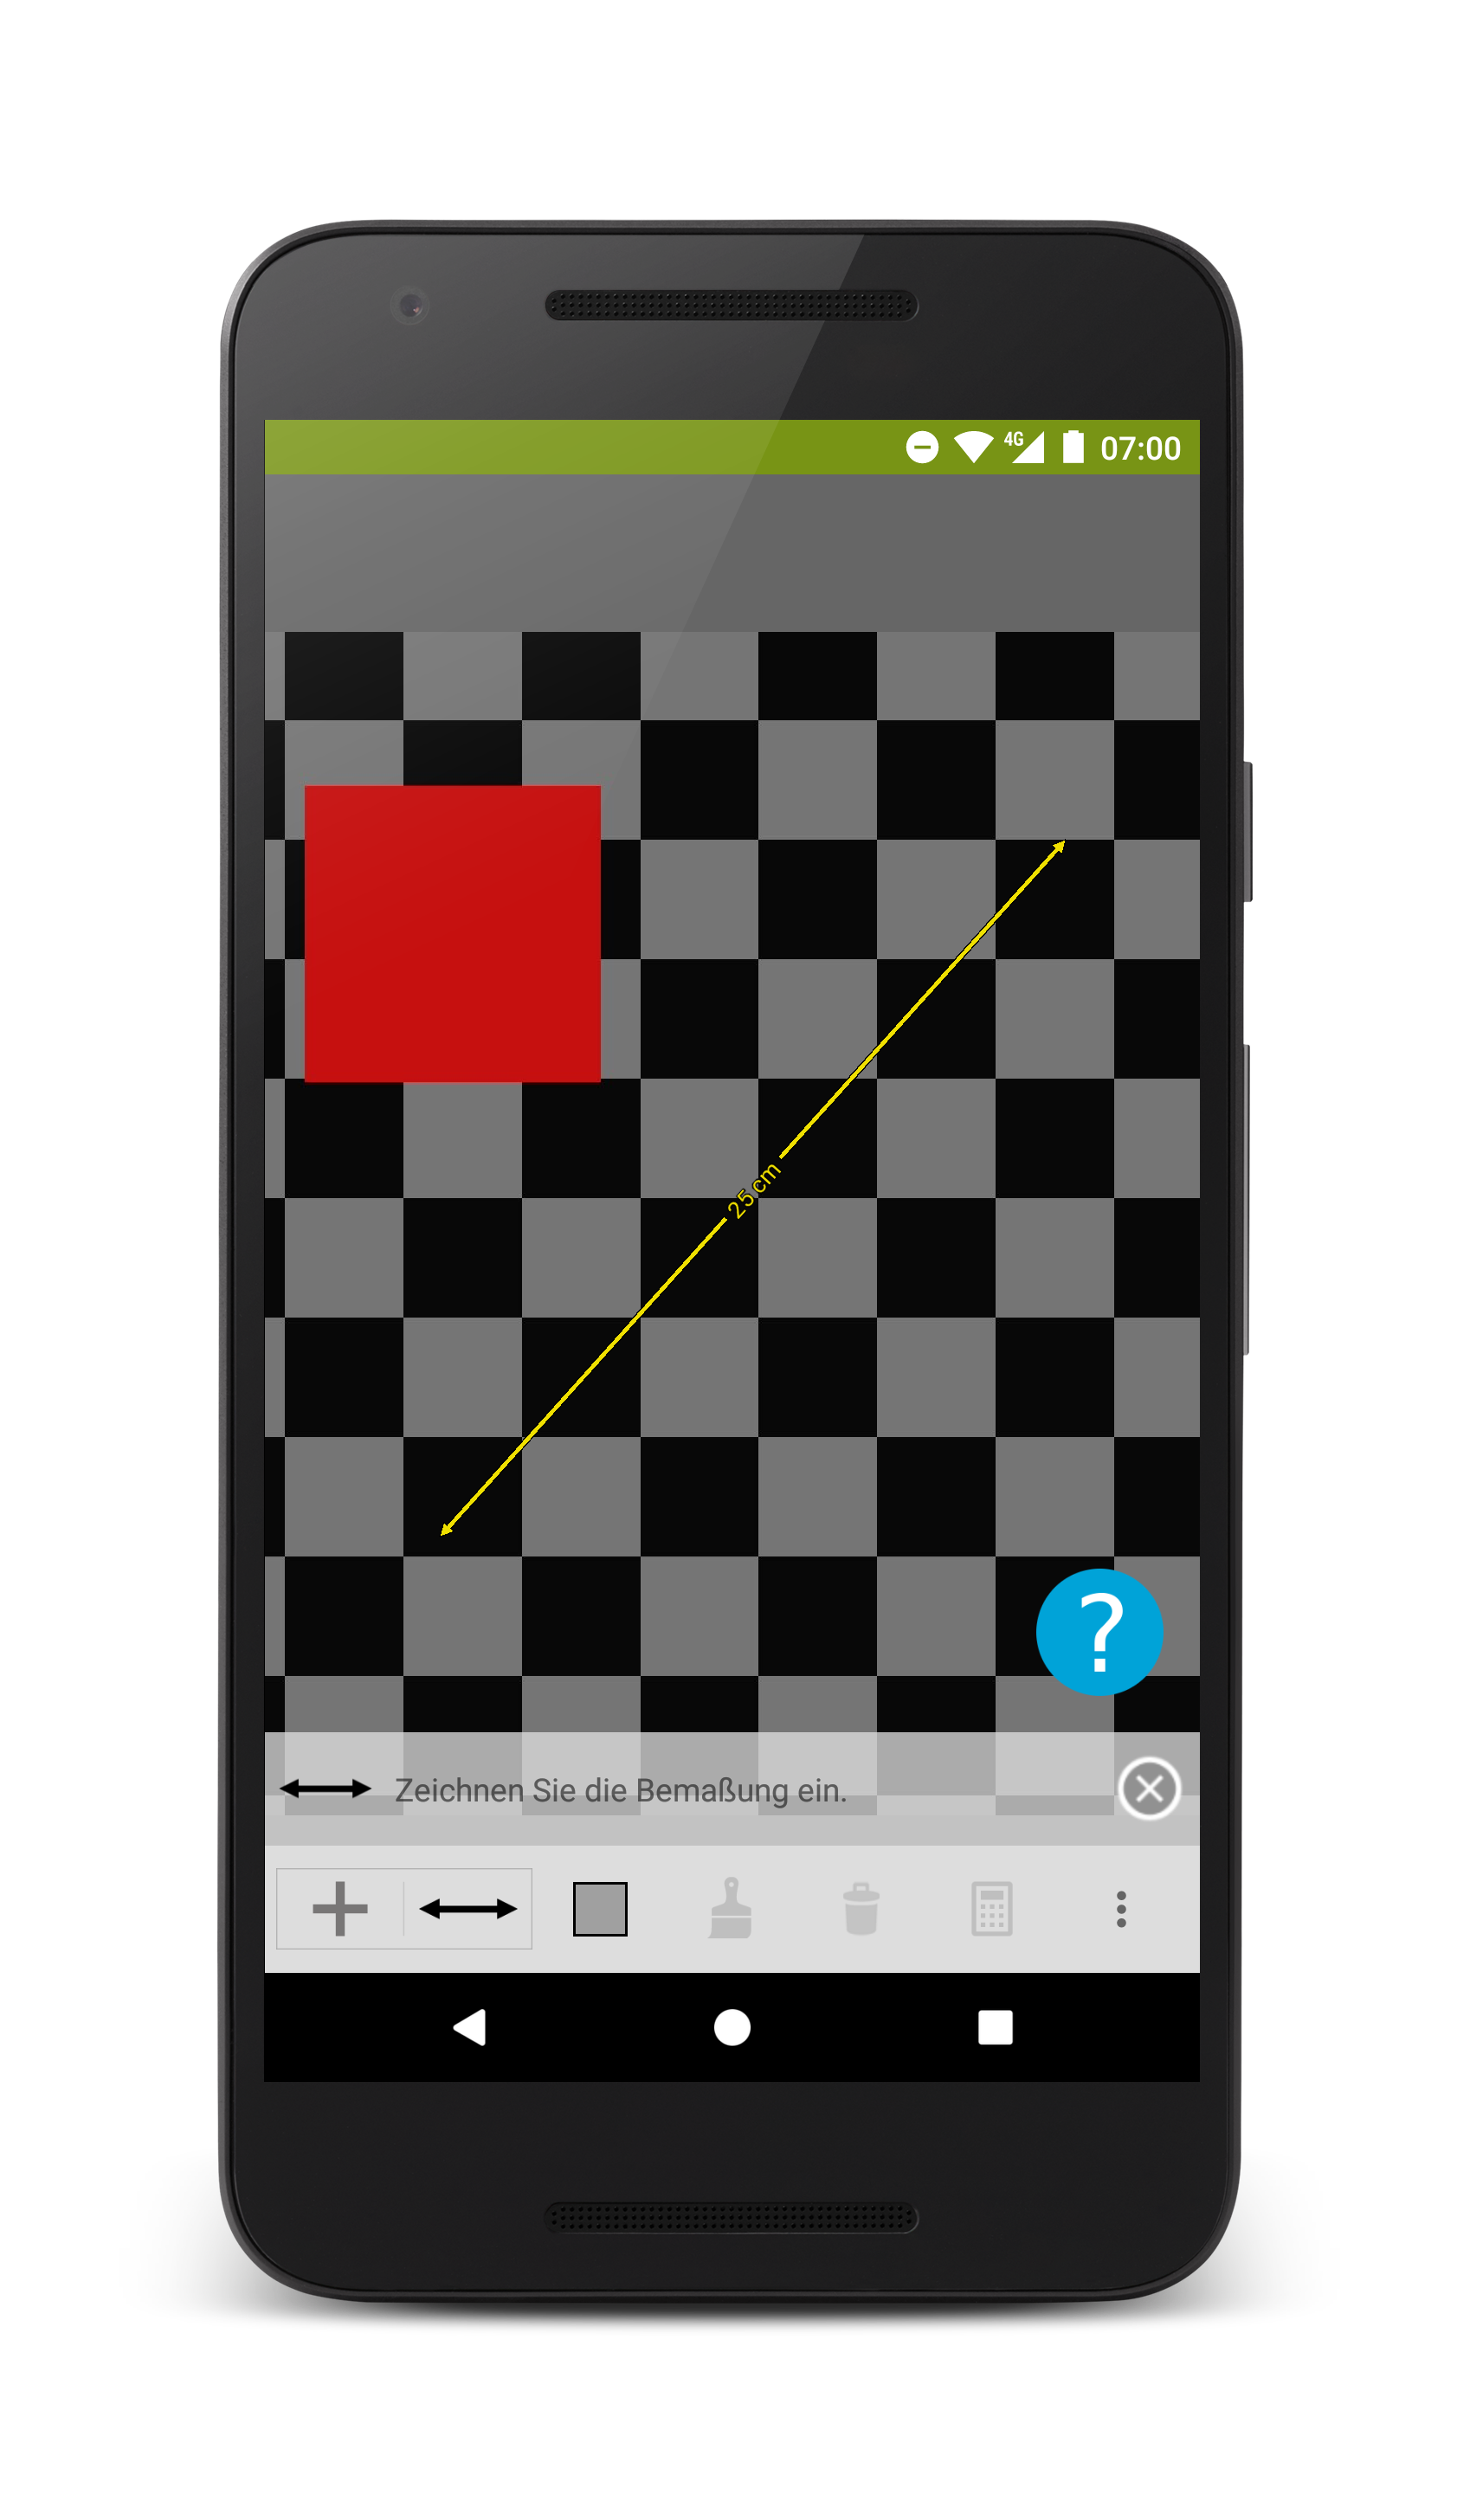
\includegraphics[keepaspectratio, width=\textwidth]{image_meter/draw}
    \caption{Aufmaße-Funktion mit eingezeichneter Form} 
    \label{fig:imdraw}	
  \end{subfigure}
  \caption{\im{} nach dem Start der App und in der Aufmaß-Funktion}
\end{figure}

\noindent
Zudem kann der Nutzer über die Statusleiste die gewünschte Form und deren Farbe auswählen.
Bereits eingezeichnete Formen können im Nachhinein wieder vergrößert bzw. verkleinert und in ihrem Aussehen verändert werden. \\

Des Weiteren werden nur die Funktionen, die zum jeweiligen Systemzustand ausführbar sind (z.B. Löschen und Textändernungen nur wenn Form ausgewählt), in der Statusleiste angezeigt.
Die App bietet die Möglichkeit aus sieben Formen - zehn in der Pro-Version - auszuwählen, und diese in das Bild einzuzeichnen.
Zusätzlich kann man in dieser App Gebrauch von Referenzpunkten machen, die es der App ermöglichen, neu eingezeichnete Formen automatisch mit Messwerten zu versehen.
Versehentlich ausgeführte Aktionen können durch einen Undo- bzw. Redo-Button in der Statusleiste rückgängig gemacht bzw. wiederholt werden. \\

Auch in dieser App lassen sich gespeicherte Bilder zu einem späteren Zeitpunkt weiter bearbeiten.
Außerdem können mehrere Bilder gleichzeitig zusammen in einer \emph{PDF} exportiert werden.

\subsubsection{Evaluation}\label{subsec:imeva}

Hilfe und Dokumentation (Nielsen~\autoref{itm:N10}) werden in dieser App in Form des ``Tipp des Tages'' Dialogs (siehe \autoref{fig:imtip}), welcher sich zum Start der App zeigt, und durch eine dedizierte Benutzeroberfläche, die man über den Floating Action Button erreicht, bereit gestellt.

\begin{wrapfigure}{R}{0.5\textwidth}
  \centering
  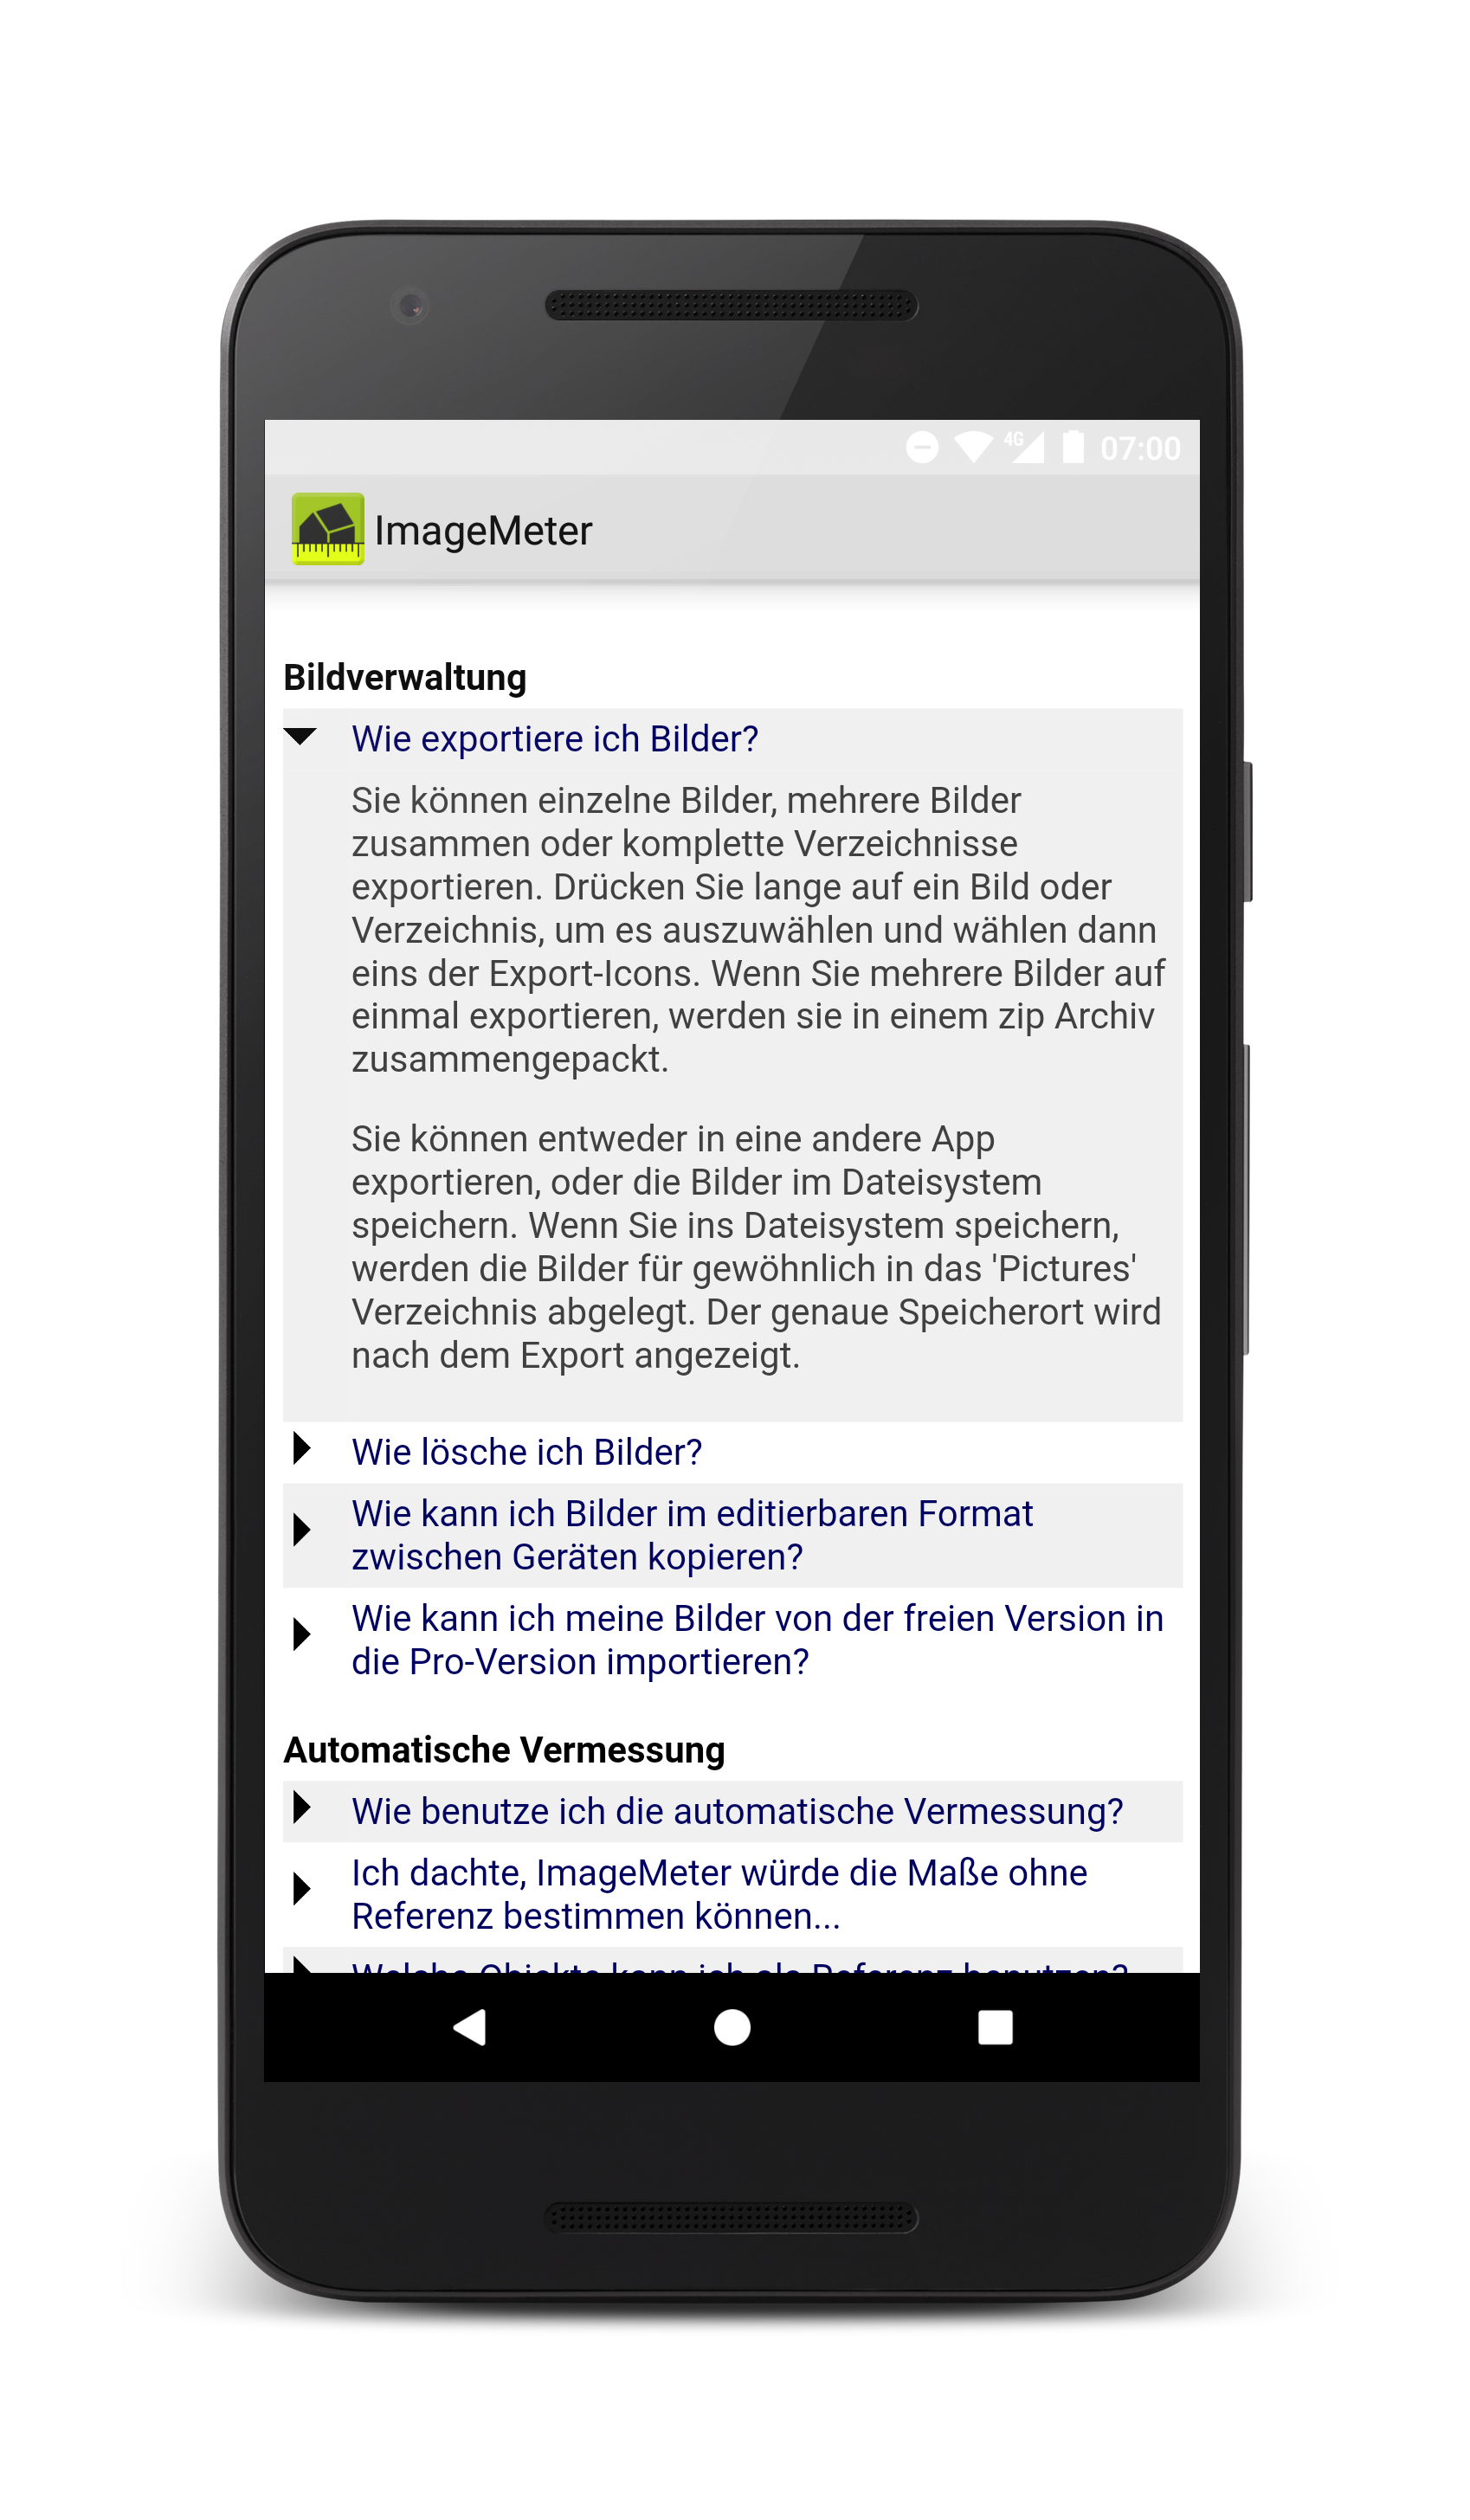
\includegraphics[keepaspectratio, width=0.5\textwidth]{image_meter/faq}
  \caption{Hilfeoberfläche der App}
  \label{fig:imfaq}
\end{wrapfigure}

Hierbei bietet die Hilfeoberfläche Antworten auf eine vorgegebene Menge Fragen zu den verschiedenen Funktionen der App (siehe \autoref{fig:imfaq}). \\

Die Statusleite zeigt zu jedem Zeitpunkt den ausgewählten Modus und die verfügbaren Aktionen an, und gibt dem Benutzer so eine angemessene und verständliche Rückmeldung über den aktuellen Systemzustand der App (Nielsen~\autoref{itm:N1} \& \autoref{itm:N5}). \\

Formen können, nachdem sie in das Bild gezeichnet wurden, zu einem späteren Zeitpunkt in ihrem Aussehn und ihrer Größe verändert werden. Zusätzlich dazu gibt es in den Einstellungen der App weitere Punkte, um diese den eigenen Benutzungsbedürfnissen anzupassen.
So kann zum Beispiel eingestellt werden, ob Maßeinheiten angezeigt werden sollen, welche metrischen Einheiten benutzt werden sollen, oder wie viele Dezimalstellen für Messwerte verwendet werden solle.
Dies erlaubt nicht nur eine flexible Benutzung der App, sondern sorgt gleichzeitig für eine potentielle Effizienzsteigerung, da die App nur einmal zu Beginn der Benutzung den Vorstellungen entsprechend konfiguriert werden muss (Nielsten~\autoref{itm:N7}) \\

Die App versucht Situationen, in denen Fehler auftreten könnten, präventiv zu vermeiden.
Hierzu werden Aktionen, die beim Ausführen im aktuellen Systemzustand zu einem Fehler führen würden, ausgegraut und sind nicht auswählbar (Nielsen~\autoref{itm:N5} \& \autoref{itm:N9}).

\begin{wrapfigure}{R}{0.5\textwidth}
  \centering
  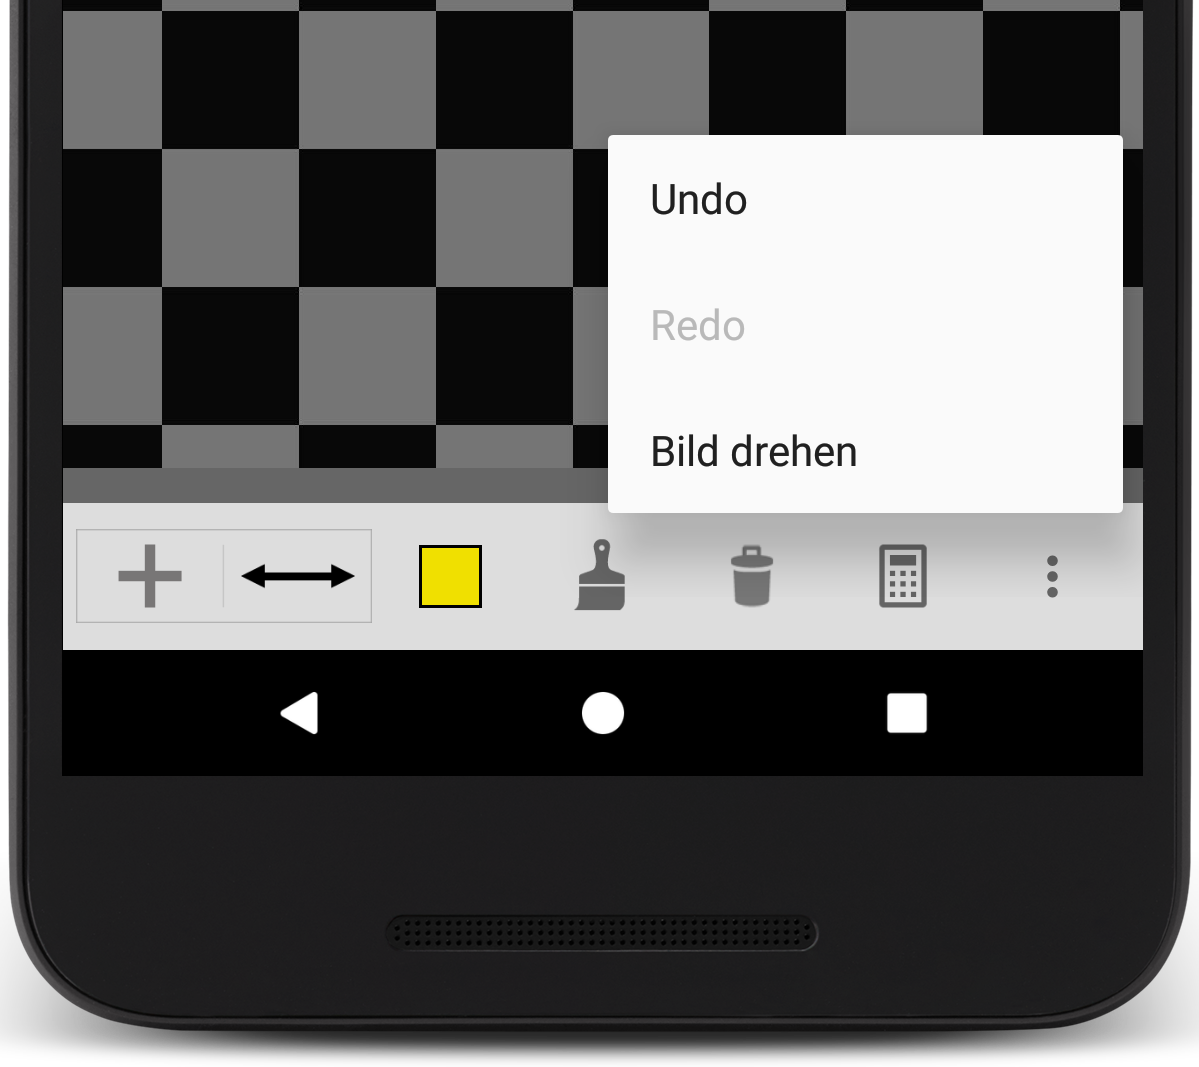
\includegraphics[keepaspectratio, width=0.5\textwidth]{image_meter/bar}
  \caption{Statusleiste in der Aufmaßfunktion}
  \label{fig:imbar}
\end{wrapfigure}

Das Ausgrauen der unbenutzbaren Aktionen führt jedoch in Kombination mit den anderen verwendeten Farben in der Statusbar schnell zu Verwirrung.
So werden hier zwei verschiedene Grautöne benutzt, die sich nur minimal unterscheiden (siehe \autoref{fig:imbar}). \todo{bisschen mehr hierzu} \\

Über einen Undo- bzw. Redo-Menüpunkt hat der Benutzer die Möglichkeit, ungewollte oder fehlerhafte Eingaben zu revidieren, oder Aktionen zu wiederholen (Nielsen \autoref{itm:N3}).
Bei der Benutzung im Hochformat sind diese Menüpunkte jedoch nicht offensichtlich erkennbar, da sie in dem Overflow-Menü \todo{def} an der rechten Seite der Statusbar versteckt sind (siehe \autoref{fig:imbar}).
Der Benutzer muss hier also durch Zufall schon einmal das Overflow-Menü ausgeklappt haben, um zu wissen, dass sich dort die Optionen zum Undo bzw. Redo befinden. \\

Ein positiver Aspekt dagegen liegt beim adäquaten Umgang mit Unterbrechungen, sowie der Unterstützung verschiedener Bildschirmausrichtungen (Nielsen~\autoref{itm:N11} \& \autoref{itm:N15}).
Beim Pausieren und Drehen der App gehen keine Informationen, wie bereits eingezeichnete Formen oder eingetragene Messwerte verloren, und das Bild bleibt stets in der erwarteten Ausrichtung. 

\begin{wrapfigure}{R}{0.5\textwidth}
  \centering
  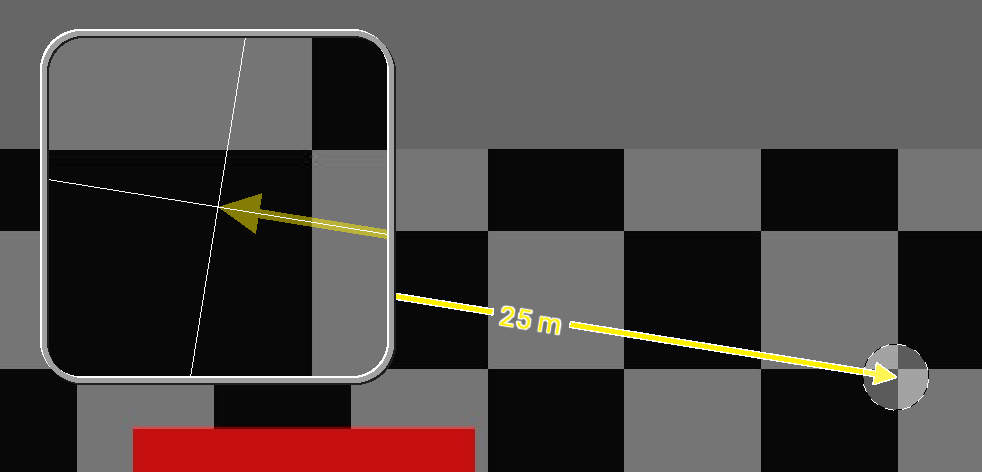
\includegraphics[keepaspectratio, width=0.5\textwidth]{image_meter/lensebug}
  \caption{Zoom-Linse verdeckt Zeichenbereich}
  \label{fig:imlense}
\end{wrapfigure}

Hinzukommend wird der zusätzliche Bildschirmplatz der sich im Querformat ergibt genutzt, um alle Elemente der Statusleiste anzuzeigen, ohne Aktionen im Overflow-Menü zu verstecken. \\

Eine positive Benutzererfahrung ergibt sich aus der einfachen und effizienten einhändigen Handhabung in Kombination mit einer fehlerfreien Gesten-Unterstützung zur Navigation im Bild. (Nielsen~\autoref{itm:N13}, \autoref{itm:N16} \& \autoref{itm:N17}). \\

Außerdem bedient sich auch diese App beim Zeichnen von Formen einer Zoom-Linse, welche den Bereich um die Fingerposition vergößert darstellt.
Negativ fällt bei der Umsetzung dieser Funktion jedoch auf, dass die Zoom-Linse statisch in der oberen linken Ecke angezeigt wird, und sich bei Kollision mit dem Zeichenfinger nicht bewegt.
Dies kann dazu führen, dass der gezoomte Bereich beim Zeichnen die Form verdeckt und seine eigentlichen Aufgabe als Hilfestellung zur genaueren und schnelleren Zeichnung verfehlt (siehe \autoref{fig:imlense}). \\

Die App ermöglicht das Teilen von vorhandenen Bildern in diese, bietet beim Exportieren jedoch keine Möglichkeit die eingetragenen Messwerte als Meta-Daten beizubehalten.
So wäre es zwar möglich, Bilder aus der bestehenden Android-App an \im{} zu teilen, diese zu bearbeiten und anschließend abzuspeichern. 
Aber es gäbe keine Möglichkeit aus der bestehenden Android-App auf die eingetragenen Messwerte zuzugreifen, und diese für einen nachgeschalteten Diesnt aufzubereiten. \\

Zusammenfassend kann gesagt werden, dass die App \im{} von \emph{Dirk Farin} die Nielsen-Heuristiken überwiegend positive erfüllt.
Die versteckten Undo/Redo-Funktionalität und die Verwirrung des Nutzers durch die Verwendung ähnlicher Grautöne für unterschiedliche Aktionen in der Statsubar sind bei der Evaluation als Negativaspekte identifiziert worden.
Besonders diese beiden Punkte in Kombination mit der fehldenden Einführung bzw. Hilfe-Stellung beim ersten Start der Aufmaß-Funktion, wirken sich negativ auf die initiale Benutzererfahrung der App aus.
So muss der Benutzer, falls sich Fragen während des Einzeichnens von Formen ergeben, die aktuelle Oberfläche verlassen, in eine andere Oberfläche wechseln, und dort die passende Frage suchen. 

Hierdurch können Fehler entstehen, die mit der Nutzung einer Android-App für die Aufmaßerfassung verhindert werden sollten.
